\documentclass[aspectratio=169,11pt]{beamer}
\usetheme{Madrid}
\usecolortheme{seahorse}
\usefonttheme{professionalfonts}
\usepackage{amsmath,amssymb,bm,booktabs,array,graphicx,hyperref,multicol}
\usepackage{tikz}
\usetikzlibrary{positioning,arrows.meta,shapes.geometric,calc}
\usepackage{xcolor,xeCJK,fontspec}
\graphicspath{{../outputs/}}
\setmainfont{texgyreheros-regular.otf}[BoldFont=texgyreheros-bold.otf,ItalicFont=texgyreheros-italic.otf]
\setsansfont{texgyreheros-regular.otf}[BoldFont=texgyreheros-bold.otf,ItalicFont=texgyreheros-italic.otf]
\setmonofont{lmmono10-regular.otf}[BoldFont=lmmonolt10-bold.otf]
\setCJKmainfont{FandolHei-Regular.otf}
\setCJKsansfont{FandolHei-Regular.otf}
\setCJKmonofont{FandolFang-Regular.otf}
\definecolor{myblue}{RGB}{36,88,135}
\definecolor{mygreen}{RGB}{40,120,80}
\definecolor{mygray}{RGB}{90,90,90}
\definecolor{myorange}{RGB}{180,100,30}
\setbeamercolor{title}{fg=myblue}
\setbeamercolor{frametitle}{fg=myblue}
\setbeamercolor{structure}{fg=myblue}
\setbeamercolor{block title}{bg=myblue,fg=white}
\setbeamercolor{block body}{bg=blue!5,fg=black}
\setbeamercolor{alertblock title}{bg=myorange,fg=white}
\setbeamercolor{alertblock body}{bg=orange!8,fg=black}
\setbeamercolor{exampleblock title}{bg=mygreen,fg=white}
\setbeamercolor{exampleblock body}{bg=green!6,fg=black}
\setbeamertemplate{navigation symbols}{}
\setbeamertemplate{footline}[frame number]
\newcommand{\R}{\mathbb{R}}
\newcommand{\sigmoid}{\sigma}
\title[Week 7]{Week 7: Phase-aware GNN 与高召回三相 N-1 筛查}
\subtitle{Topology-aware graph learning for unbalanced microgrid security prediction}
\author{ECE Course: Physics-informed AI for Microgrid Security Prediction}
\date{}
\begin{document}

\begin{frame}\titlepage\end{frame}

\begin{frame}{本周学习目标}
\begin{enumerate}
  \item 把三相微电网表示为 bus-level graph。
  \item 构造 phase-channel node features、edge features 和 global features。
  \item 用 contingency mask 编码 line outage、PV trip、BESS trip 和 PCC outage。
  \item 实现一个不依赖 PyTorch Geometric 的 message-passing GNN。
  \item 证明 graph tensor、mask、split、loss 和 metric 代码正确。
  \item 使用 high-recall threshold 和 top-k ranking 做 AI-assisted N-1 screening。
\end{enumerate}
\end{frame}

\begin{frame}{八周项目中的位置}
\centering
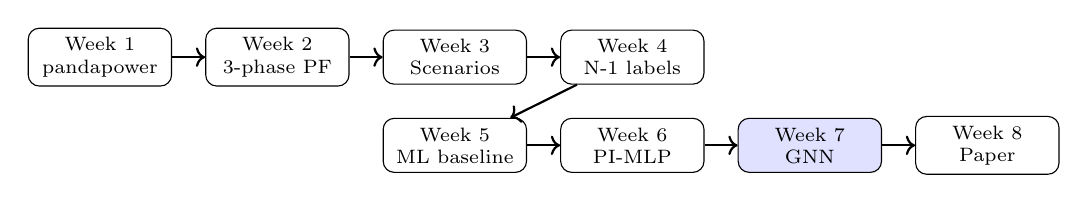
\begin{tikzpicture}[node distance=0.42cm, every node/.style={font=\scriptsize}]
\tikzstyle{box}=[draw, rounded corners, minimum width=1.82cm, minimum height=0.56cm, align=center]
\node[box] (w1) {Week 1\\pandapower};
\node[box, right=of w1] (w2) {Week 2\\3-phase PF};
\node[box, right=of w2] (w3) {Week 3\\Scenarios};
\node[box, right=of w3] (w4) {Week 4\\N-1 labels};
\node[box, below=of w3] (w5) {Week 5\\ML baseline};
\node[box, right=of w5] (w6) {Week 6\\PI-MLP};
\node[box, right=of w6, fill=blue!12] (w7) {Week 7\\GNN};
\node[box, right=of w7] (w8) {Week 8\\Paper};
\draw[->, thick] (w1)--(w2); \draw[->, thick] (w2)--(w3); \draw[->, thick] (w3)--(w4);
\draw[->, thick] (w4)--(w5); \draw[->, thick] (w5)--(w6); \draw[->, thick] (w6)--(w7); \draw[->, thick] (w7)--(w8);
\end{tikzpicture}
\vspace{0.25cm}
\begin{block}{Week 7 的角色}
把 flattened features 升级为 topology-aware graph input，并把 high-recall screening 扩展到 top-k contingency ranking。
\end{block}
\end{frame}

\begin{frame}{从 Feature Vector 到 Graph}
\begin{columns}
\begin{column}{0.48\textwidth}
\textbf{Week 5/6 表格模型}
\[
\hat y=f_\theta(\mathbf f(x_t,c))
\]
\begin{itemize}
  \item 一行样本对应一组 features。
  \item 拓扑位置需要手工编码。
  \item line outage 下游影响不显式。
\end{itemize}
\end{column}
\begin{column}{0.50\textwidth}
\textbf{Week 7 图模型}
\[
\hat y=f_\theta(G_{t,c})
\]
\begin{itemize}
  \item bus 是节点，line 是边。
  \item A/B/C 三相信息是 node channels。
  \item outage mask 改变 message passing。
\end{itemize}
\end{column}
\end{columns}
\end{frame}

\begin{frame}{为什么 Microgrid 适合 GNN}
\begin{itemize}
  \item line outage 风险与 feeder 拓扑、下游负荷、上游供电路径强相关。
  \item PV/BESS trip 的风险不仅取决于容量，也取决于接入位置。
  \item VUF 风险依赖 A/B/C 三相负荷和 DER 的空间分布。
  \item PCC outage 是 system-level contingency，需要全局图状态。
\end{itemize}
\begin{block}{核心动机}
GNN 不是替代 pandapower，而是作为三相 N-1 全扫描前的快速候选排序器。
\end{block}
\end{frame}

\begin{frame}{图学习问题定义}
给定 operating scenario $x_t$ 和 contingency $c_k$：
\[
G_{t,k}=\left(\mathcal N,\mathcal E, X_t, E_k, g_{t,k}\right)
\]
\begin{itemize}
  \item $X_t\in\R^{N\times F_x}$：bus-level phase-channel node features。
  \item $E_k\in\R^{2L\times F_e}$：directed edge features and outage mask。
  \item $g_{t,k}\in\R^{F_g}$：scenario、base-case security、contingency metadata。
  \item $y_{t,k}\in\{0,1\}$：Week 4 violation label。
\end{itemize}
\[
\hat p_{t,k}=\Pr(y_{t,k}=1\mid G_{t,k})
\]
\end{frame}

\begin{frame}{教学版 Feeder Graph}
\centering
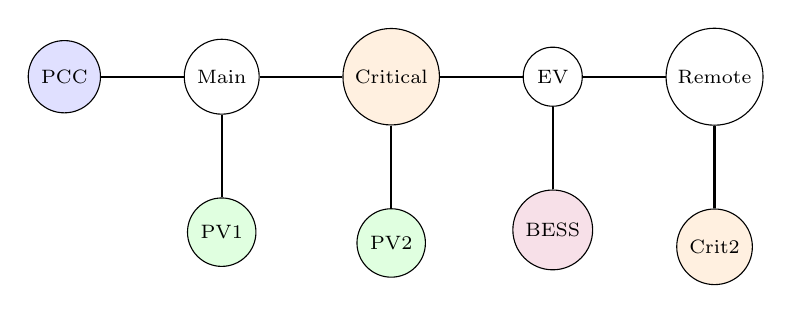
\begin{tikzpicture}[node distance=1.05cm, every node/.style={font=\scriptsize}]
\tikzstyle{bus}=[circle, draw, minimum size=0.75cm, align=center]
\node[bus, fill=blue!12] (pcc) {PCC};
\node[bus, right=of pcc] (main) {Main};
\node[bus, right=of main, fill=orange!12] (crit) {Critical};
\node[bus, right=of crit] (ev) {EV};
\node[bus, right=of ev] (remote) {Remote};
\node[bus, below=of main, fill=green!12] (pv1) {PV1};
\node[bus, below=of crit, fill=green!12] (pv2) {PV2};
\node[bus, below=of ev, fill=purple!12] (bess) {BESS};
\node[bus, below=of remote, fill=orange!12] (crit2) {Crit2};
\draw[thick] (pcc)--(main)--(crit)--(ev)--(remote);
\draw[thick] (main)--(pv1); \draw[thick] (crit)--(pv2); \draw[thick] (ev)--(bess); \draw[thick] (remote)--(crit2);
\end{tikzpicture}
\vspace{0.2cm}
\begin{block}{MVP 设计}
9 个 buses，8 条 undirected lines，转换为 16 条 directed edges。该拓扑足够小，便于学生逐项检查 tensor 和 mask。
\end{block}
\end{frame}

\begin{frame}{Bus-level Phase-channel 表示}
\begin{block}{节点仍然是 bus}
不是把每个 bus 拆成 $(i,a),(i,b),(i,c)$ 三个相节点，而是把 A/B/C 信息放入同一个 bus 的特征向量。
\end{block}
\begin{exampleblock}{示例 node features}
\small
is\_pcc, is\_critical, is\_pv\_bus, is\_bess\_bus;\newline
$P^{load}_a,P^{load}_b,P^{load}_c$; $P^{PV}_a,P^{PV}_b,P^{PV}_c$;\newline
$P^{BESS,dis}_a,P^{BESS,dis}_b,P^{BESS,dis}_c$;\newline
$P^{BESS,ch}_a,P^{BESS,ch}_b,P^{BESS,ch}_c$; contingency flags and bus depth.
\end{exampleblock}
\end{frame}

\begin{frame}{Phase-level GNN 是后续扩展}
\begin{columns}
\begin{column}{0.48\textwidth}
\textbf{本周 MVP：bus-level}
\begin{itemize}
  \item 节点数量小。
  \item 实现简单。
  \item 适合一周课程。
  \item A/B/C 作为 channels。
\end{itemize}
\end{column}
\begin{column}{0.48\textwidth}
\textbf{论文扩展：phase-level}
\begin{itemize}
  \item 节点为 $(i,a),(i,b),(i,c)$。
  \item 更自然表示单相 DER。
  \item 需要建模相间耦合。
  \item 适合期刊扩展。
\end{itemize}
\end{column}
\end{columns}
\end{frame}

\begin{frame}{Contingency Encoding}
\small
\begin{tabular}{ll}
\toprule
Contingency & Graph encoding \\
\midrule
line outage & edge availability $a_{ij}=a_{ji}=0$，并标记端点 bus \\
PV trip & 标记 PV bus，加入 PV trip global flag \\
BESS trip & 标记 BESS bus，加入 BESS trip global flag \\
PCC outage & 标记 PCC bus，加入 no-slack / PCC outage global flag \\
\bottomrule
\end{tabular}
\vspace{0.3cm}
\begin{block}{同一个 scenario，多张 graph}
同一 operating scenario 下，不同 contingency 对应不同 $E_k$ 和 $g_{t,k}$，因此模型可以给不同故障排序。
\end{block}
\end{frame}

\begin{frame}{Message Passing 方程}
\[
h_i^{(0)}=\phi_x(x_i)
\]
\[
m_{ij}^{(r)}=a_{ij}\,\psi_\theta\left(h_j^{(r)},e_{ij}\right)
\]
\[
h_i^{(r+1)}=\sigma\left(W_s h_i^{(r)}+\sum_{j\in\mathcal N(i)}m_{ij}^{(r)}\right)
\]
\begin{itemize}
  \item $a_{ij}=1$：line available，message passes。
  \item $a_{ij}=0$：line outage，message blocked。
\end{itemize}
\end{frame}

\begin{frame}{Graph-level Readout}
经过 $K$ 层 message passing 后：
\[
h_G=\mathrm{mean}_{i\in\mathcal N}h_i^{(K)}
\]
拼接 global features：
\[
z=[h_G,g_{t,k}]
\]
输出 unsafe probability：
\[
\hat p_{t,k}=\sigmoid(w^\top z+b)
\]
\begin{block}{为什么用 mean pooling}
mean pooling 简单、稳定、对节点排列不敏感，适合作为教学版 graph-level classifier。
\end{block}
\end{frame}

\begin{frame}{FlattenedMLP Baseline}
为了公平比较，本周还训练一个非图模型：
\[
\mathbf z=\mathrm{flatten}(X,E,g),\qquad \hat p=\mathrm{MLP}(\mathbf z)
\]
\begin{itemize}
  \item 输入信息量与 GNN 接近。
  \item 不显式使用 edge index 和 message passing。
  \item 用来判断 topology-aware inductive bias 是否带来收益。
\end{itemize}
\begin{alertblock}{注意}
小数据集上 FlattenedMLP 可能表现更好；这不是失败，而是实验解释的一部分。
\end{alertblock}
\end{frame}

\begin{frame}{Dataset Interface}
Week 7 读取 Week 4/5 输出：
\begin{itemize}
  \item week5\_outputs\_complete/week5\_ml\_input\_dataset.csv
  \item week4\_outputs\_complete/week4\_contingency\_table.csv
\end{itemize}
每一行仍是 $(x_t,c_k,y_{t,k},s_{t,k})$，但会转换为：
\begin{itemize}
  \item $X_{node}$: $[n_{samples}, n_{bus}, n_{node\ features}]$;
  \item $E_{edge}$: $[n_{samples}, n_{directed\ edges}, n_{edge\ features}]$;
  \item $G_{global}$: $[n_{samples}, n_{global\ features}]$。
\end{itemize}
\end{frame}

\begin{frame}{No-leakage 原则}
\begin{columns}
\begin{column}{0.48\textwidth}
\textbf{允许输入}
\begin{itemize}
  \item scenario settings；
  \item base-case voltage/VUF/loading；
  \item static topology；
  \item device placement；
  \item contingency identity/location。
\end{itemize}
\end{column}
\begin{column}{0.48\textwidth}
\textbf{禁止输入}
\begin{itemize}
  \item post-contingency voltage；
  \item post-contingency loading；
  \item post-contingency VUF；
  \item violation flags；
  \item severity score；
  \item convergence/service-loss label。
\end{itemize}
\end{column}
\end{columns}
\end{frame}

\begin{frame}{Graph Tensor Proof}
Notebook 检查：
\begin{itemize}
  \item graph connected；
  \item graph radial: $|\mathcal E|=|\mathcal N|-1$；
  \item directed edge count: $2|\mathcal E|$；
  \item node / edge / global tensors finite；
  \item edge availability 和 outage flag 保持二元。
\end{itemize}
\begin{exampleblock}{执行结果}
\[
X: (77,9,26),\quad E:(77,16,6),\quad G:(77,16)
\]
\end{exampleblock}
\end{frame}

\begin{frame}{Contingency Mask Proof}
\begin{itemize}
  \item line outage：恰好两个 directed edges 被置为 unavailable；
  \item non-line contingencies：PV/BESS/PCC 不改变 line availability；
  \item PV trip：恰好标记一个 PV bus；
  \item BESS trip：恰好标记 BESS bus；
  \item PCC outage：恰好标记 PCC bus。
\end{itemize}
\begin{block}{为什么重要}
如果 mask 错了，GNN 学到的是错误拓扑；即使指标好，也没有工程可信度。
\end{block}
\end{frame}

\begin{frame}{Permutation-invariance Proof}
Graph-level prediction 不应依赖任意 bus 排列：
\[
\hat p(G)=\hat p(\pi(G))
\]
其中 $\pi$ 同时重排 node tensor 并 remap edge index。
\begin{block}{Notebook 检查}
随机选择一个样本，随机重排 bus order，并用 remapped edge index 重新预测。
\end{block}
\begin{exampleblock}{通过标准}
$|\hat p(G)-\hat p(\pi(G))| < 10^{-6}$。
\end{exampleblock}
\end{frame}

\begin{frame}{训练协议}
\begin{enumerate}
  \item Random holdout: train / validation / test。
  \item Scaler 只在 training samples 上 fit。
  \item Validation set 选择 high-recall threshold。
  \item Test set 只报告最终结果。
  \item Group CV 检查 unseen scenario 和 unseen contingency。
\end{enumerate}
\[
\max_\tau\ \mathrm{PFCallsSaved}_{val}(\tau)
\quad \mathrm{s.t.}\quad
\mathrm{Recall}_{val}(\tau)\ge 0.95
\]
\end{frame}

\begin{frame}{High-recall Screening Metrics}
\small
\begin{tabular}{ll}
\toprule
Metric & Meaning \\
\midrule
Recall & unsafe contingencies sent to detailed PF \\
FNR & missed unsafe fraction \\
Precision & fraction of screened-positive cases that are truly unsafe \\
PF calls saved & cases predicted safe and skipped \\
Missed violations & false negatives; most safety-critical number \\
AUPRC & useful under class imbalance \\
Top-k recall & dangerous contingencies covered by top-$k$ ranking \\
\bottomrule
\end{tabular}
\vspace{0.25cm}
\begin{alertblock}{安全筛查核心}
准确率不是核心。漏报 unsafe contingency 才是最危险的错误。
\end{alertblock}
\end{frame}

\begin{frame}{Top-k Contingency Ranking}
对每个 scenario：
\begin{enumerate}
  \item 计算所有 candidate contingencies 的 risk score；
  \item 按 score 从高到低排序；
  \item 只对 top-$k$ contingencies 运行三相 PF；
  \item 统计 violation recall@$k$。
\end{enumerate}
\[
\mathrm{Recall@}k=\frac{\#\{\text{unsafe contingencies in top-}k\}}{\#\{\text{unsafe contingencies}\}}
\]
\begin{block}{避免自评泄漏}
Notebook 使用 scenario-group out-of-fold scores 做 top-k ranking。
\end{block}
\end{frame}

\begin{frame}{训练曲线}
\centering
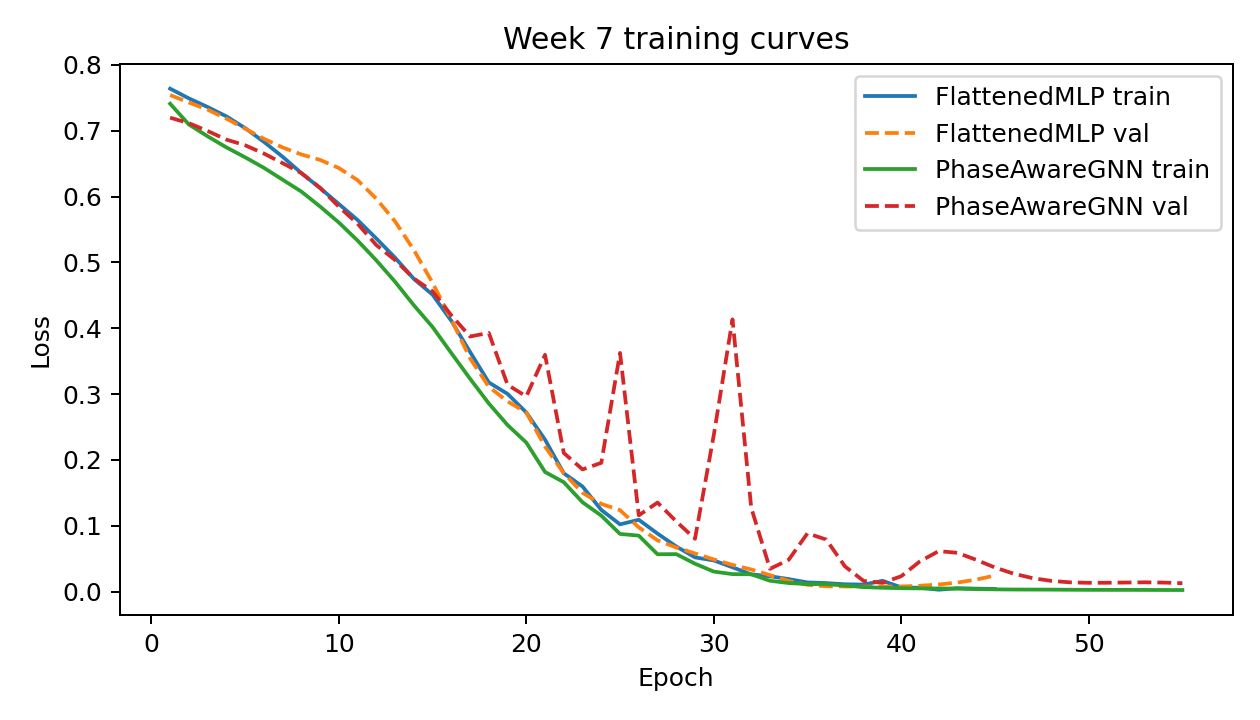
\includegraphics[width=0.80\textwidth]{week7_training_curves.png}
\end{frame}

\begin{frame}{Precision-Recall 曲线}
\centering
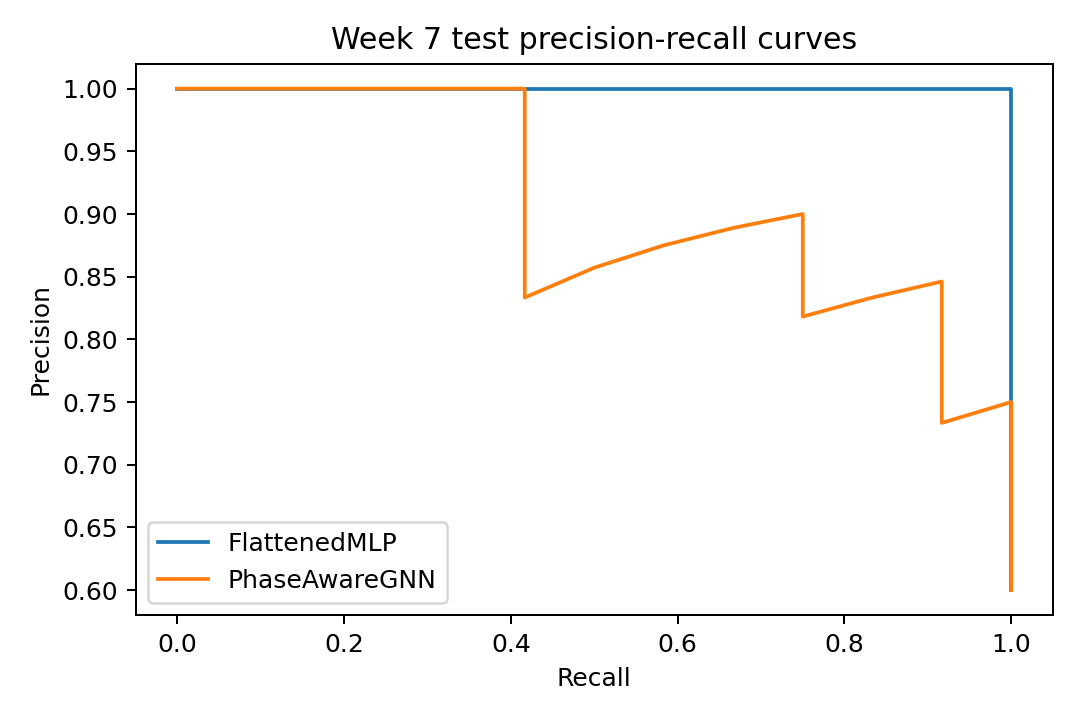
\includegraphics[height=0.76\textheight,keepaspectratio]{week7_precision_recall_curves.png}
\end{frame}

\begin{frame}{Saved PF Calls vs Missed Violations}
\centering
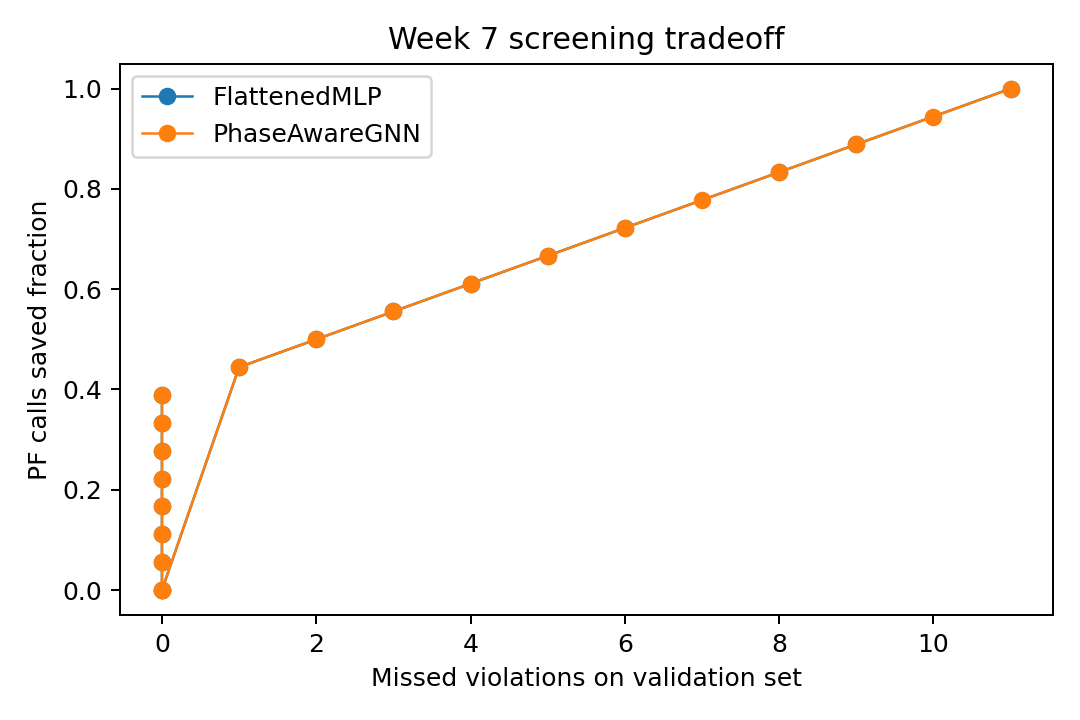
\includegraphics[height=0.76\textheight,keepaspectratio]{week7_saved_calls_vs_missed_violations.png}
\end{frame}

\begin{frame}{Random Holdout 结果}
\centering
\scriptsize
\begin{tabular}{lrrrrrr}
\toprule
Model & Recall & Precision & FNR & Saved & Missed & AUPRC \\
\midrule
FlattenedMLP & 1.000 & 1.000 & 0.000 & 0.400 & 0 & 1.000 \\
PhaseAwareGNN & 0.583 & 0.875 & 0.417 & 0.600 & 5 & 0.913 \\
\bottomrule
\end{tabular}
\vspace{0.25cm}
\begin{alertblock}{如何解释}
教学数据只有 77 个样本。这里 MLP 更强，说明当前 flattened features 已经很有信息量，而 GNN 需要更多 scenarios、更多拓扑或更强正则化才能稳定体现优势。
\end{alertblock}
\end{frame}

\begin{frame}{OOD-style Group CV}
\centering
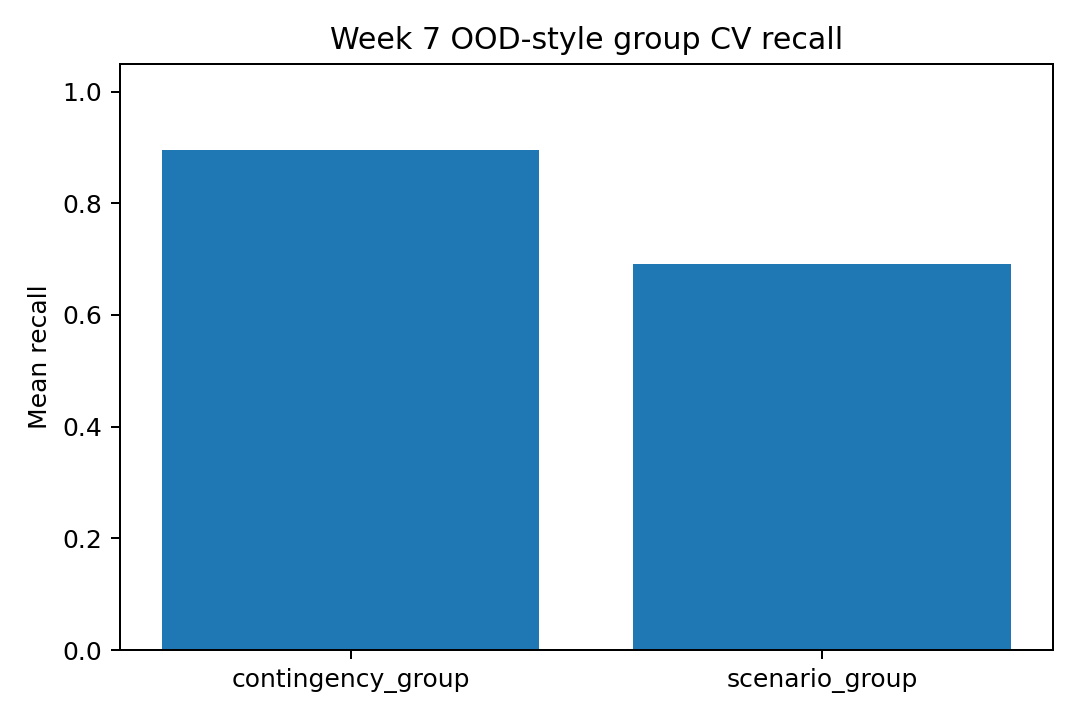
\includegraphics[width=0.74\textwidth]{week7_group_cv_recall.png}
\end{frame}

\begin{frame}{Group CV 摘要}
\centering
\scriptsize
\begin{tabular}{lrrrrr}
\toprule
CV type & Folds & Mean recall & Mean precision & Mean FNR & Missed \\
\midrule
Scenario-group & 7 & 0.690 & 0.739 & 0.310 & 18 \\
Contingency-group & 11 & 0.896 & 0.665 & 0.104 & 8 \\
\bottomrule
\end{tabular}
\vspace{0.3cm}
\begin{block}{结论}
Unseen scenario 比 unseen contingency 更难，说明 operating condition diversity 是后续数据集扩展的重点。
\end{block}
\end{frame}

\begin{frame}{Top-k Violation Recall}
\centering
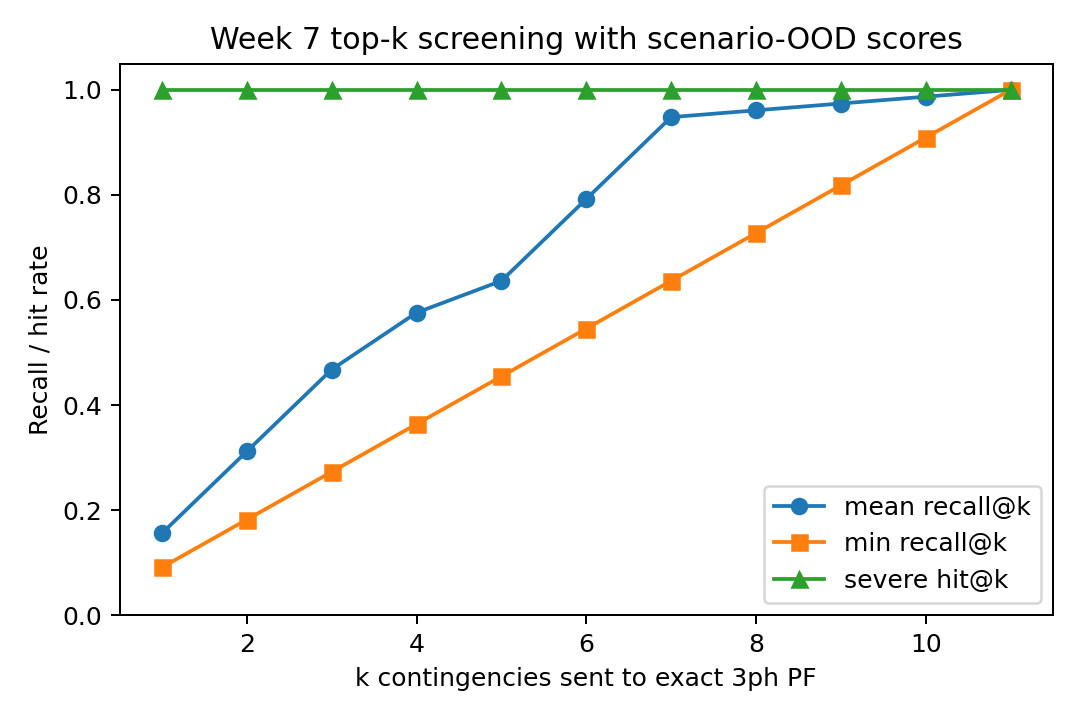
\includegraphics[height=0.76\textheight,keepaspectratio]{week7_topk_violation_recall.png}
\end{frame}

\begin{frame}{Top-k 结果解读}
\scriptsize
\centering
\begin{tabular}{rrrr}
\toprule
$k$ & PF call fraction & Mean recall@$k$ & Severe hit@$k$ \\
\midrule
1 & 0.091 & 0.156 & 1.000 \\
3 & 0.273 & 0.468 & 1.000 \\
5 & 0.455 & 0.636 & 1.000 \\
7 & 0.636 & 0.948 & 1.000 \\
8 & 0.727 & 0.961 & 1.000 \\
11 & 1.000 & 1.000 & 1.000 \\
\bottomrule
\end{tabular}
\vspace{0.3cm}
\begin{block}{操作含义}
在该教学数据上，若每个 scenario 只扫描 top-7 contingencies，平均可覆盖约 95 percent unsafe contingencies，同时减少约 36 percent PF calls。
\end{block}
\end{frame}

\begin{frame}{Validation Suite}
Notebook 保存 44 项 validation checks：
\begin{multicols}{2}
\begin{itemize}
  \item base graph connected;
  \item radial topology;
  \item directed edge count;
  \item finite tensors;
  \item line outage mask;
  \item PV/BESS/PCC flags;
  \item no post-contingency leakage;
  \item split disjoint;
  \item preprocessing finite;
  \item forward shape;
  \item finite loss / gradients;
  \item permutation invariance;
  \item group CV disjoint;
  \item top-k finite.
\end{itemize}
\end{multicols}
\begin{exampleblock}{执行结果}
$44/44$ checks passed.
\end{exampleblock}
\end{frame}

\begin{frame}{代码结构}
\small
\begin{enumerate}
  \item Load Week 4/5 datasets。
  \item Define teaching microgrid graph。
  \item Construct node, edge, global features。
  \item Run graph tensor and no-leakage proofs。
  \item Split and scale train/val/test。
  \item Define FlattenedMLP and PhaseAwareGNN。
  \item Run permutation-invariance proof。
  \item Train holdout models and select threshold。
  \item Run scenario/contingency group CV。
  \item Compute top-k ranking using OOF scores。
  \item Save tables, figures, validation summary。
\end{enumerate}
\end{frame}

\begin{frame}{论文中的 Contribution 表述}
\begin{block}{稳妥写法}
We propose a phase-aware graph representation for three-phase microgrid N-1 security screening, where bus-level phase channels, line outage masks, and contingency-specific global features are combined in a message-passing classifier.
\end{block}
\begin{block}{避免过度表述}
不要写：GNN always outperforms MLP。\newline
可以写：GNN provides a topology-aware prototype; superiority requires larger and more diverse feeders/scenarios.
\end{block}
\end{frame}

\begin{frame}{Ablation 建议}
后续可在 Week 8 或论文扩展中加入：
\begin{itemize}
  \item 去掉 phase channels，只保留 total load/PV；
  \item 去掉 outage edge mask，只保留 contingency ID；
  \item mean pooling vs max pooling vs mean+max pooling；
  \item line outage only vs all contingency types；
  \item bus-level graph vs phase-level graph；
  \item 更多随机 operating scenarios。
\end{itemize}
\end{frame}

\begin{frame}{Limitations}
\begin{itemize}
  \item 当前数据集只有 7 scenarios 和 77 N-1 samples。
  \item 当前 feeder topology 单一，不能证明跨 feeder 泛化。
  \item Bus-level phase channels 还没有显式表示相间耦合。
  \item GNN 在小数据下可能不如 strong tabular baseline。
  \item 真正部署前仍需三相 PF 作为最终验证。
\end{itemize}
\begin{alertblock}{科研态度}
安全应用中，AI screening 应该减少计算量，而不是跳过必要的工程验证。
\end{alertblock}
\end{frame}

\begin{frame}{Week 7 到 Week 8 的衔接}
Week 8 将把 Weeks 4--7 组织成 mini-paper：
\begin{itemize}
  \item Week 4：三相 N-1 label generation；
  \item Week 5：traditional ML baseline；
  \item Week 6：physics-informed / limit-aware MLP；
  \item Week 7：phase-aware GNN and top-k screening；
  \item Week 8：paper figures、tables、method diagram、limitations。
\end{itemize}
\begin{block}{最终论文主线}
Fast but conservative AI-assisted screening for unbalanced microgrid N-1 static security assessment.
\end{block}
\end{frame}

\begin{frame}{课堂练习}
\begin{enumerate}
  \item 把 GNN 的 mean pooling 改为 max pooling。
  \item 去掉 cont\_line\_endpoint node flag，只保留 edge outage mask。
  \item 去掉 A/B/C phase channels，只使用 total load/PV。
  \item 把 hidden dimension 从 48 改为 16、32、96。
  \item 用 scenario-group OOF scores 画每个 scenario 的 top-k ranking 表。
  \item 设计 phase-level graph 的节点和边。
\end{enumerate}
\end{frame}

\begin{frame}{本周交付物}
\begin{itemize}
  \item 完整 clean notebook：课堂运行。
  \item executed notebook：教师检查与复现。
  \item 输出表：holdout results、group CV、top-k recall、validation summary。
  \item 输出图：training curves、PR curves、saved calls tradeoff、top-k recall。
  \item Week 8 可直接引用的 GNN method 和 limitation 表述。
\end{itemize}
\end{frame}

\end{document}
